%\documentclass{article}

\documentclass[9pt,twocolumn,twoside,lineno]{gsajnl}
\usepackage{amsmath}
% Use the documentclass option 'lineno' to view line numbers

\articletype{preprint} % article type
% {inv} Investigation 
% {gs} Genomic Selection
% {goi} Genetics of Immunity 
% {gos} Genetics of Sex 
% {mp} Multiparental Populations

%Simulating Isolation by Distance in Continuous Space
%Space is the Place: How Dispersal and Competition Shape Genetic Variation in Continuous Space
%Impacts of Continuous Spatial Structure on Analyses of Population Genetic Data
\title{Impacts of Isolation by Distance on Demographic Modeling and Association Studies}

\author[$\ast$,1]{C.J. Battey}
\author[$\ast$]{Peter Ralph}
\author[$\ast$]{Andrew Kern}

\affil[$\ast$]{University of Oregon Dept. Biology, Institute for Ecology Evolution}
\keywords{Space; Population Structure; Demography; Haplotype block sharing}

\runningtitle{SPACENESS} % For use in the footer 

%% For the footnote.
%% Give the last name of the first author if only one author;
% \runningauthor{FirstAuthorLastname}
%% last names of both authors if there are two authors;
% \runningauthor{FirstAuthorLastname and SecondAuthorLastname}
%% last name of the first author followed by et al, if more than two authors.
\runningauthor{Battey \textit{et al.}}

\begin{abstract}
Individuals exist in continuous space, but standard models in population genetics are based on discrete randomly-mating populations exchanging migrants. As the availability of population-level whole genome data allows inference of increasingly fine-scale patterns of ancestry in many species, models incorporating realistic demographic and spatial processes are needed to accurately describe spatial structure and control for its impacts on analyses of selection and demography. Here we implement a forward-time simulation of evolution in continuous space and use it to study the impacts of dispersal and density-dependent competition on population genetic summary statistics, demographic inference, and association studies. Low dispersal slows the geographic spread of ancestry and increases branch lengths corresponding to mid-frequency alleles because of slow coalescence among distant groups of individuals. As a result demographic inference from the site frequency spectrum is biased towards inferring a turbulent past demographic history and a recent decline in populations when neighborhood sizes are below 20. For many common population genetic summary statistics the variation associated with different sampling strategies is larger than that observed across the range of dispersal distances we simulated, pointing to the need to carefully account for the spatial distribution of sampling when interpreting results. Last we show that spatially correlated environments cause genome-wide signals of association with purely environmental phenotypes in linear-regression GWAS, and this bias is not fully corrected by regressing out principal components positions during the analysis.  
\end{abstract}

\begin{document}

\maketitle
\thispagestyle{firststyle}
\marginmark
\firstpagefootnote


\correspondingauthoraffiliation{1}{301 Pacific Hall, University of Oregon Dept. Biology, Institute for Ecology and Evolution. cbattey2@uoregon.edu.}
\vspace{-35pt}% Only used for adjusting extra space in the left column of the first page

\section{Introduction}
The inescapable reality that biological organisms live, move, and reproduce in continuous spatial landscapes has been all but ignored in population genetic models. 

In most sexual organisms individuals mate with other nearby individuals, leading to a positive correlation between genetic and geographic distances. This pattern of "isolation by distance" \citep{Wright1943} is one of the most widely replicated empirical findings in population genetics \citep{Chen2017,Jay2012,Sharbel2000}, but is only heuristically approximated by existing forward-time models of molecular evolution based on discrete demes exchanging migrants. As the availability of population-level whole-genome data allows inference of increasingly fine-scale patterns of ancestry in many species, models incorporating biologically realistic demographic and spatial processes are needed to accurately describe continuous spatial structure and control for its impacts on analyses of selection and demography. This situation is particularly clear in human population genetics, where individual ancestries are often interpreted as mixtures of discrete populations in part because of modeling assumptions underlying discrete clustering algorithms and association analyses are often strongly dependent on statistical corrections for population stratification \citep{Berg2018,Bulik-Sullivan2015,Young2018,Heckerman2016,Kang2010,Sohail2018}.  

The best-studied approaches to population genetics in continuous space were developed by \citep{Wright1943} and \citep{Malecot1948}, who derived expressions for genetic differentiation in continuous space assuming Poisson distributed numbers of offspring and independent dispersal among individuals. A key finding of Wright's model is that many important aspects of continuous populations can be described in terms of "neighborhood size" -- the number of potential mates for an individual in a given generation, defined as $4\pi\sigma^2d$, where $\sigma$ is the average dispersal distance and $d$ is population density. \cite{Maruyama1972} found that the rate of decline in genetic diversity in a 2-dimensional continuous population shifts between distinct regimes when $D\sigma^2$ is greater or less than 1, and proposed that this had the important implication that most population genetic expectations for randmoly mating populations could be applied to continuously distributed populations with relatively little error. 

Though some aspects of continuous populations are fairly well described by the Wright-Malécot models, \cite{Felsenstein1975} showed that the assumptions of independent dispersal and Poisson distributed offspring that are the basis of these models are incompatible. Over time, a population meeting them will clump into a small number of geographic clusters occupying only a part of the available range. Although real populations are often clumped on landscapes due to factors like varying habitat quality and competition among species, the Wright and Malécot models produce much more extreme clumping than is observed in real organisms and fail to account for the density-dependent declines in population growth rate that are widely observed in real populations (CITE). 

One method for modeling populations in continuous space is then to assume the existence of a grid of discrete randomly-mating populations connected by migration, which prevents clustering by forcing all regions to be occupied in every generation. Among many other important results drawn from this class of "lattice" or "stepping stone" models, \cite{Rousset1997} showed that the slope of the a linear regression of genetic differentiation ($F_{st}$) against the logarithm of spatial distance is an estimate of neighborhood size. Though good approximations of continuous structure given high dispersal (Barton(?)), these models are not truly continuous, force a uniform realized population density across landscapes, and limit investigation of spatial structure below the level of the deme. An alternative method is to model the geographic spread of ancestry backwards in time through a diffusion approximation -- an approach that has recently made significant progress in modeling both dispersal and demographic parameters \citep{Barton2010,Kelleher2014,Ringbauer2017,Ringbauer2018}. However these models currently lack a well-described forward-time analog that produces biologically realistic spatial patterns and are subject to the same difficulty in incorporating selection and other biological processes as all other reverse time methods (CITE??).

We took a direct approach to the clustering problem of classical forward-time models by incorporating density dependence into the model. By scaling the probability of survival in each timestep to local population density we shift reproductive output towards regions of low-density and prevent populations from clustering. A similar approach was taken previously by \citep{Doebeli2003} who used an individual based model with continuous space and density dependent fitness to study the probability of speciation along continuous environmental gradients. However to our knowledge all previous implementations of continuous space models have focused on a small number of genetic loci as the unit of analysis, which limits the ability to investigate the impacts of continuous space on genome-wide genetic variation as is now routinely sampled from real organisms. 

Here we describe an implementation of an individual-based model in continuous space that incorporates overlapping generations, a Gaussian dispersal kernel, and density-dependent fitness. The model scales to chromosome-scale alignments across tens of thousands of individuals, and outputs the full genealogy and recombination history of all final-generation individuals. We use this simulation to describe how sampling strategy interacts with isolation by distance to cause systematic variation in population genetic summary statistics typically analyzed under discrete population models. We then examine how the fine-scale spatial structures occurring under limited dispersal impact demographic inference from the site frequency spectrum; finding that inflation of branch lengths for mid-frequency alleles associated with slow coalescence of distant individuals can bias analyses towards inferring turbulent demographic histories and recent declines in population size. 

Last, we use our model to study the impacts of isolation by distance in continuous space on genome-wide association studies (GWAS). Variation in ancestry proportions between case and control cohorts is expected to cause inflation of test statistics at SNPs with different allele frequencies among populations \citep{Price2006}. Because most phenotypes are influenced by the environment and environmental factors are often spatially correlated, subtle spatial structure within continuous populations can also deflate $p$ values in GWAS of quantitative traits \citep{Mathieson2012}. These issues are particularly prominent for polygenic traits, because the deflated $p$ values expected from polygenic phenotype correlations are superficially similar to those expected from population structure \citep{Bulik-Sullivan2015,Young2018}. However most studies examining the effects of stratification on GWAS have focused on simulating phenotypes for real genotype data \citep{Price2006,Bulik-Sullivan2015} or generating simulated genotypes by sampling from static allele frequency distributions \citep{Bulik-Sullivan2015,Heckerman2016}. These approaches address application to human data but are not based on a true generative model and so provide limited insight into the processes generating stratification bias in association analyses. Here we simulate both the underlying genealogy and phenotypes of a continuously distributed population and seek to identify regions of parameter space -- i.e. the strength of isolation by distance and the spatial distribution of environmental effects on phenotypes -- in which common methods of stratification bias corrections in GWAS are subject to bias. 

%[move some of this to methods, rewrite to avoid repitition w above]  A common method of correcting for population structure in GWAS is to run a principal components analysis on the genotype matrix and include PC coordinates as covariates in a linear regression for each SNP \citep{Price2006}. Mixed model GWAS employs a different statistical framework but takes a similar approach by incorporating a kinship matrix describing pairwise genetic relatedness among samples as a random effect in a linear mixed model \citep{Yu2006,Kang2008}. In both approaches the key question is whether or not the ancestry components of the model adequately describe "background" levels of genetic variation in the sample relative to any confounding effects of ancestry and phenotype. Recent studies in European and British populations \citep{Kerminen2018,Berg2018,Sohail2018} have found evidence of residual population stratification in effect size estimates from large-scale GWAS employing both linear and mixed model approaches, suggesting that existing structure corrections may be inadequate. For traits controlled by a few large effect loci this confounding effect is likely to be relatively small, but for analyses of complex traits with thousands of putatively associated SNPs the potential for confounding is high. Here we simulate a range of spatially correlated phenotypes for simulated individuals and seek to identify conditions under which existing GWAS structure corrections are subject to bias caused by continuous population structure.  

\section{Materials and Methods}
\label{sec:materials:methods}

\subsection{A Forward-Time Model of Evolution in Continuous Space}

We implemented our model using the non-Wright-Fisher module in the program SLiM v3.0 \citep{Haller2019}. Each time step consists of three stages: reproduction, dispersal, and competition. To reduce the parameter space we use the same parameter, denoted $\sigma$, to modulate the spatial scale of interactions at all three stages by adjusting the standard deviation of the corresponding Gaussian functions. As in previous work \citep{Wright1943,Ringbauer2017}, $\sigma$ as applied in our dispersal step is approximately equal to the mean parent-offspring distance.  

At the beginning of the simulation individuals are distributed randomly on a continuous landscape. Mates are selected proportional to distances among individuals weighted by a Gaussian function with mean $1/(2\pi\sigma^2)$ and standard deviation $\sigma$. Wright's \cite{Wright1943} "Neighborhood Size", defined as $4\pi\sigma^2 K$ where $K$ is the population density, is then the approximate number of individuals available for mating in our simulation. The number of offspring is drawn from a Poisson distribution with mean $1/L$, where $L$ is the average lifespan. If new offspring are produced, we simulate dispersal by taking two draws from a normal distribution with mean 0 and standard deviation $\sigma$ and adding these to the x and y coordinates of the first parent. 

Density-dependent competition is simulated by adjusting the probability of survival of each individual proportional to the local density of individuals up to a distance $3\sigma$ away, scaled according to the same Gaussian function used for mate selection. Given a per-unit carrying capacity $K$ and average fecundity $F$, the probability of survival $d$ for individual $i$ after adjustment for density is:

\begin{equation}
    d_{i}=min(0.95,\frac{1}{1+\rho*\sum_{i}{G(x)}})
\end{equation}
where 
\begin{equation}
    \rho = F/((1+F)*K)
\end{equation} 
and $G(x)$ is the Gaussian function used to weight distances to other individuals. 

A major challenge in all spatial models is dealing with range edges. When local population density is used to model competition, edge or corner populations can be assigned artificially high fitness values because they lack neighbors within their interaction radius but outside the bounds of the simulation. We approximate a decline in habitat suitability near edges by decreasing the probability of survival proportional to the square root of distance to edges in units of $\sigma$. The final probability of survival for individuals within one $\sigma$ of an edge is 

\begin{multline}
    s_{i}=d_{i} min(1,\sqrt{x_{i}/\sigma})
    min(1,\sqrt{y_{i}/\sigma})\\
    min(1,\sqrt{(x_{max}-x_{i})/\sigma})
    min(1,\sqrt{(y_{max}-y_{i})/\sigma)}
\end{multline}

where $x$ and $y$ are spatial coordinates. 

To isolate spatial effects from other components of the model such as overlapping generations, increased variance in reproductive success, and density-dependent fitness, we  also implemented a second version of the SLiM simulation in which mates are selected at random and offspring disperse to a random location on the landscape. For all simulations the full genealogy and recombination history of final-generation individuals were stored as tree sequences \citep{Kelleher2018}. 

%We compared our model output to a two-dimensional stepping-stone model and a one-population coalescent model implemented in msprime \citep{Kelleher2016}. To isolate spatial effects from other components of the model such as overlapping generations and density-dependent probability of survival, we also ran a second version of the SLiM model with random mate selection and dispersal. 

We ran 400 simulations for the spatial and random-mating SLiM models on a square landscape of size 50 with per-unit carrying capacity $K=5$ (census $N \approx 10,000$), average lifetime $L=4$, genome size $1\times10^{8}$, recombination rate $1\times10^{-9}$, and drawing $/sigma$ values from a uniform distribution bounded by 0.2 and 4. To speed up the simulations and limit memory overhead we used a mutation rate of 0 in SLiM and later applied mutations to the coalesced tree sequence with msprime's 'mutate( )' function. Because msprime assumes that timesteps are in units of generations, we divided the per-generation rate of $1\times10^{-8} mut/site/gen$ by the generation time estimated for each value of $\sigma$ (see 'Genealogical Parameters' below) to convert the rate to units of mutations/site/timestep. We then verified that this procedure produced the correct number of mutations by comparing a subset of simulations with SLiM-generated mutations (which are applied only at mating events) with mutations added by msprime (Supplementary Figure 1). Simulations were run for 1.6 million timesteps (approximately 30N generations), or until all extant individuals shared a common ancestor within the simulation (i.e. the tree sequence had coalesced). 

%Coalescent stepping-stone simulations were on a 5x5 grid with 10 haploid samples per deme and migration between adjacent populations. To facilitate comparison across simulation types we ran one coalescent simulation for every SLiM parameter set. Because $\sigma$ is approximately equal to the mean distance between parent and offspring, we approximate the relationship between $\sigma$ and the migration rate in a grid simulation as $\sigma=4md$, where $m$ is the migration rate and $d$ is the ratio of landscape widths in continuous space vs coalescent simulations (here, 10). That is, an individual in an interior population has a $4m$ probability of being a migrant, and if it is a migrant will move $d$ units on the map. We set the total $N_{e}$ equal to the census size of each SLiM simulation divided by the variance in reproductive output (see below). 

\subsection{Sampling}
Unlike reverse time approaches our model records the genealogy and sequence variation of the complete population, but in real populations genotypes are only observed from a subset of individuals. We modeled three sampling strategies meant to approximate common data collection methods in empirical genetic studies (Figure 1). "Random" sampling selects individuals at random from across the full landscape. "Point" sampling selects individuals proportional to their distance from four equally spaced points on the landscape. Last, "midpoint" sampling selects individuals in proportion to their distance from the middle of the landscape. In practice random sampling is rarely conducted because of the difficulty of accessing all parts of a species range and the inefficiency of collecting only single individuals at all sites. Point and midpoint sampling strategies are both common, particularly for species that require traps or collecting stations to be set up and dismantled at every site.  

\subsection{Genealogical Parameters}
To study the geographic spread of genealogical ancestry in our simulations we output the full pedigree of all individuals over 50 generations with $\sigma$ set to 0.2, 0.35, 0.5, 1, 2, and 3.5 (corresponding to Wright's Neighborhood Sizes of 2.5, 7.7, 15.7, 62.8, 251.3, and 769.7, respectively). We then selected the individual closest to the center of the landscape in the final generation of each simulation, pruned the pedigree to include only its genealogical ancestors (that is, regardless of the amount of genetic material actually inherited from a given ancestor) and plotted the age of its most recent ancestor in each region of the full landscape using the 2-dimensional summary feature of ggplot2 in R \citep{Wickham2016}. We calculated the rate of spread of genealogical ancestry by estimating the mean and maximum distances between the focal individual and its ancestors in each generation and then fitting a linear model for distance as a function of generations using ordinary least squares regression. 

We also estimated the variance in offspring and generation time for all simulations. To estimate generation times we stored the age of all parents for 200 timesteps and took the mean. To estimate variance in offspring we output the complete pedigree of all individuals in SLiM, counted the number of offspring for all individuals born in timesteps 50-150 (to ensure that the simulation captured the full lifespan of the sampled individuals), and calculated the variance. 

\subsection{Summary Statistics}
We calculated a set of 20 summary statistics (Supplementary Table 1) from 60 diploid individuals sampled randomly from the final generation of each simulation using the python package scikit-allel \citep{Miles2017}. Statistics included common single-population summaries such as mean pairwise divergence ($\pi$), inbreeding coefficient ($F_{is}$), and Tajima's D, as well as the classic isolation-by-distance regression of genetic distance ($D_{xy}$) against the logarithm of geographic distances \citep{Rousset1997}, which we summarized as the correlation coefficient between $log10(spatial distance)$ and the proportion of identical base pairs among individuals. 

Following recent studies that showed strong signals for dispersal and demography in the distribution of shared haplotype block lengths \citep{Ringbauer2017,Baharian2016}, we also calculated various summaries of the distribution of pairwise identical-by-state (IBS) block lengths among samples. Intuitively, haplotype block length distributions should contain more information about the genealogy of a set of samples than allele frequency measures alone because they reflect the influence of two Poisson processes (mutation and recombination) acting along its branches, rather than just one. 

The full distribution of lengths of IBS tracts for each pair of individuals was first calculated with a custom python function. We then calculated the first three moments of this distribution (mean, variance, and skew) and the number of blocks over $1e6$ base pairs both for each pair of individuals and for the full distribution across all pairwise comparisons. To assess the degree to which the IBS tract length distribution shifts with spatial distance, we then estimated correlation coefficients between spatial distance and each moment of the pairwise IBS tract distribution. Because more closely related individuals on average share longer haplotype blocks we expect that spatial distance will be negatively correlated with mean haplotype block length, and that this correlation will be strongest (i.e. most negative) when dispersal is low. The variance, skew, and count of long haplotype block statistics are meant to reflect the relative length of the right (upper) tail of the distribution, which represents the frequency of long haplotype blocks and is thus most informative of recent demographic events \citep{Ringbauer2017} (cite Coop \& Ralph here \& above). 

\subsection{Demographic Modeling}
We fit single-population demographic models to the site frequency spectra of 20 individuals from each spatial SLiM simulation with the program Stairwayplot \citep{Liu2015}. This analysis was replicated across random, point, and midpoint sampling strategies. Site frequency spectra used for input data were calculated in scikit-allel \citep{Miles2017}. 100 bootstrap replicates were generated for each simulation by resampling over sites. Models were then fit across all bootstrap replicates using default settings in Stairwayplot and the median estimate of $Ne$ per generation was used to represent the output of each simulation. The resulting inferred population size histories were plotted with line colors scaled to $\sigma$ to visualize how dispersal scaling impacts estimates of demographic history.  

\subsection{Association Studies}
To assess the degree to which spatial structure confounds GWAS we simulated four types of nongenetic phenotype variation for 1000 randomly sampled individuals in each spatial SLiM simulation and conducted a linear-regression GWAS with PC covariates in PLINK \citep{PURCELL2007}. SNPs with a minor allele frequency less than 0.5\% were excluded from this analysis. Phenotype values were meant to roughly reflect the distribution of height across Europe, which has recently been found to be confounded with population structure in large scale GWAS \citep{Berg2018,Sohail2018}. Conceptually our approach is similar to that taken in \citep{Mathieson2012}, though here we model fully continuous spatial variation and focus on genome-wide effects rather than low-frequency alleles specifically. 

In the first simulation phenotypes for all individuals were drawn from a normal distribution with mean 110 and standard deviation 10. Next we simulated clinal environmental influences on phenotype by drawing the phenotypes from independent normal distributions in which the mean was scaled by an individual's x position such that it varied by 2 standard deviations across the map. Third, we approximate concentrated environmental effects by drawing phenotypes for individuals with x and y coordinates below 20 from a normal distribution with mean 2 standard deviations above the rest of the map. Last, we simulated a "patchy" environmental influence on phenotypes by selecting 10 random points on the map and drawing phenotypes for all individuals within two map units of any selected point from a normal distribution with mean 2 standard deviations above the rest of the map. 

Principal components analysis (PCA) was conducted in scikit allel on the matrix of derived allele counts by individual for each simulation. SNPs were first filtered to remove strongly linked sites by calculating LD between all pairs of SNPs in a 200-SNP moving window and dropping one of each pair of sites with an $R^2$ over 0.1. The LD-pruned allele count matrix was then centered and all sites scaled to unit variance when conducting the PCA, following recommendations in \citep{Patterson2006}.   

We ran linear-model GWAS both with and without the first 10 principal components as covariates in PLINK and summarized results across simulations by counting the number of significant SNPs with an expected false positive rate of less than 5\% after adjusting p values with the R function p.adjust(...,method="fdr"). We also examined $p$ values for systemic inflation by estimating the expected values from a uniform distribution (because no SNPs were used when generating phenotypes), plotting observed against expected values for all simulations, and using the two-dimensional binning feature of ggplot2 \citep{Wickham2016} to find the mean $\sigma$ value in each region of quantile-quantile space. 

\section{Results}

\subsection{Genealogical Parameters and Run Times}

\subsection{Summary Statistics}
\subsubsection{Diversity}
As expected from theory based on the Wright-Malécot model \citep{Maruyama1972}, limited dispersal increases the coalescence time of a set of randomly-sampled individuals relative to a random-mating model. This is reflected in sequence data as a larger number of segregating sites and inflated estimates of expected heterozygosity ($\pi$, Figure 2). In practice the difference in segregating sites and expected heterozygosity in our simulations is negligible above neighborhood sizes of 65 ($\sigma$=1). Conversely observed heterozygosity (the fraction of heterozygous individuals) is lower than the random mating expectation when dispersal is low, and as a consequence the inbreeding coefficient ($F_{is}$) is positive. This is the continuous space version of the Wahlund effect \citep{Wahlund1928} - a deficit of heterozygous individuals when samples are drawn from subdivided populations. Similar observations of positive $F_{is}$ have been observed from stepping-stone simulations in \citep{Shirk2014} and \citep{Neel2013}.  

Tajima's $D$ is also inflated by low dispersal; reflecting a shift in the underlying genealogy in which nearby individuals coalesce quickly but distant groups of individuals take much longer to coalesce than they would under random mating. As a result the number of mid-frequency alleles is inflated, which increases expected heterozygosity relative to the count of segregating sites and leads to increased Tajima's $D$. The pattern is similar to that produced by declining population sizes, in which the terminal branches of the genealogy are short relative to those expected in constant populations. Here, however, the effect is caused by geographically limited dispersal instead of sampling from a declining population. 

\subsubection{Site Frequency Spectrum}


\subsubsection{Haplotype Block Lengths}


\subsubsection{Spatial Correlations}

Trends in pairwise haplotype block sharing parallel those seen in SNP-based diversity estimates. At low dispersal the mean length of an identical-by-state block shared between two randomly sampled individuals is lower than expected under random mating. This is because the average coalescence time of any two individuals is higher, which leaves more time for both mutation and recombination to introduce variation along a given stretch of genome.

The strongest signals of limited dispersal are in statistics that directly incorporate spatial information. The correlation coefficient between spatial distance and pairwise genetic differentiation ($D_{xy}$) is positive and declines as dispersal increases, as expected under the theory developed by \citep{Rousset1997} and others. As in \citep{Ringbauer2017} and \citep{Baharian2016} we observed that the pairwise distribution of haplotype block lengths is more strongly left-skewed under limited dispersal. In our summaries this is reflected in negative correlations between spatial distance and the mean, variance, skew, or count of long blocks from the pairwise distribution of identical-by-state block lengths. This is because individuals that are closer geographically also have more recent coalescence times when dispersal is limited, which results in fewer mutations and recombination events that can break up long shared haplotypes. Note, however, that the mean of the IBS tract length distribution has only weak signal for $\sigma$ because it is a very noisy summary of the data. The count of long haplotype blocks and the skew of the pairwise distribution (which reflects the relative length of the right tail of this distribution) appear to contain much stronger signal. 

\subsection{Demographic Modeling}



\subsection{GWAS}
Spatially correlated phenotypes in populations with low dispersal distances cause uncorrected association analyses to report significant associations at most genome-wide SNPs (Figure 1). No inflation was observed for the "normal" phenotype distribution which is random with respect to space, demonstrating that this effect is caused by the interaction of isolation by distance and spatially correlated phenotypes. The deflation in $p$ values for spatial phenotypes is particularly pronounced for the corner and clinal distributions, likely because in these cases our sample captures more phenotypic variation than in the "patchy" distribution. When PCA positions are included as covariates the vast majority of SNPs no longer pass a 5\% FDR significance threshold, but up to 1000 genome-wide significant hits (out of an average of 150,000 SNPs) were observed even in relatively high dispersal simulations for the corner and clinal distributions. 

Notably, many SNPs inferred as significant are in close proximity along the genome and likely reflect haplotypes that became common in one region of the landscape (Figure 1, supplementary figures X) [note: add example manhattan plots for s=0.3 and s=3 to fig, supp figs for manhattan plots across a larger range of sigma]. Thus the assumption that patterns of linkage disequilibrium are uncorrelated with allele frequency differentiation, which is the basis of LD score regression \citep{Bulik-Sullivan2015}, may not hold for these simulations. TODO revisit this with more quantitative analysis (need to keep genotypes to do LD scores?) 

In the case of clinal phenotypes, PCA covariates perform very well in correcting for population stratification at low dispersal distances but the correction breaks down above neighborhood sizes of 250. This pattern appears to reflect a loss of descriptive power in the first ten axes of the PCA, which describe less of the total variation in the data as neighborhood size increases (Figure 1 PANEL TO BE ADDED). Essentially, PCA loses descriptive power faster than the breakdown in correlations between allele frequencies and spatial position that our GWAS is picking up on, so eventually the statistical correction breaks down. 
Examining quantile-quantile plots shows that $p$ value deflation is most pronounced for the corner phenotype distribution and is particularly strong for simulations with neighborhood sizes of less than 20. These results are similar to the observation of high inflation for spatially discrete phenotypes in \citep{Mathieson2012}. Quantile-quantile plots of clinal and nonspatial phenotypes also show evidence of $p$ value $inflation$ (i.e. points below the 1:1 line), which is observed only when PCA covariates are included in the analysis (see Supplementary Figure X for plots of uncorrected GWAS results). This likely reflects the loss of power in GWAS when both phenotype and ancestry are correlated with space, which creates a partially confounded study design. 


\section{Discussion}

\subsection{GWAS}

% As in \citep{Mathieson2012} we observed that the deflation in $p$ values after PCA correction is largest for spatially discrete phenotypes, and is weaker for phenotypes that are clinal over space. When dispersal is low and isolation by distance is strong this effect is pronounced enough to create statistically significant associations at nearly every variable site in the genome unless statistical corrections for population structure are implemented. For strongly structure populations and phenotypes that vary systematically over space, the estimated effect sizes and biological interpretations of linear-regression GWAS are therefore controlled primarily by the method of stratification control rather than underlying causal associations between phenotype and genotype. 

%This is unlikely to be a significant issue for studies seeking to identify a small number of causal alleles as long as there is variation within populations at those sites. However analyses of putatively polygenic phenotypes may be badly affected both by deflation of $p$ values from uncontrolled stratification and by inflation of $p$ values caused by the use of PCA covariates. Though many studies now employ mixed-model methods \citep{Kang2008,Yu2006,Kang2010} which are likely more robust to stratification (though not immune, see \citep{Berg2018}), using principal components regression as the method of stratification control is still common in analyses of human genetics [quality time w nature genetics]. 

\section{Data Availability}

\section{Acknowledgements}

\begin{figure*}[p]
\centering
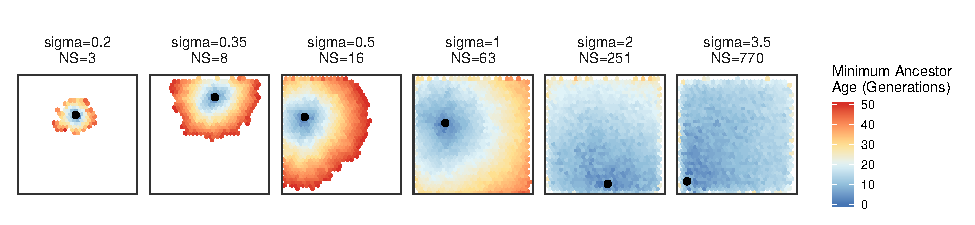
\includegraphics[width=\textwidth]{min_ancestor_age_maps.pdf}
\caption{[placeholder - working on this] Geographic spread of genealogical ancestors from a random individual over 50 generations, by Neighborhood size and $\sigma$. Colors are scaled by the age of the most recent ancestor.}
\label{fig:spectrum}
\end{figure*}

\begin{figure*}[p]
\centering
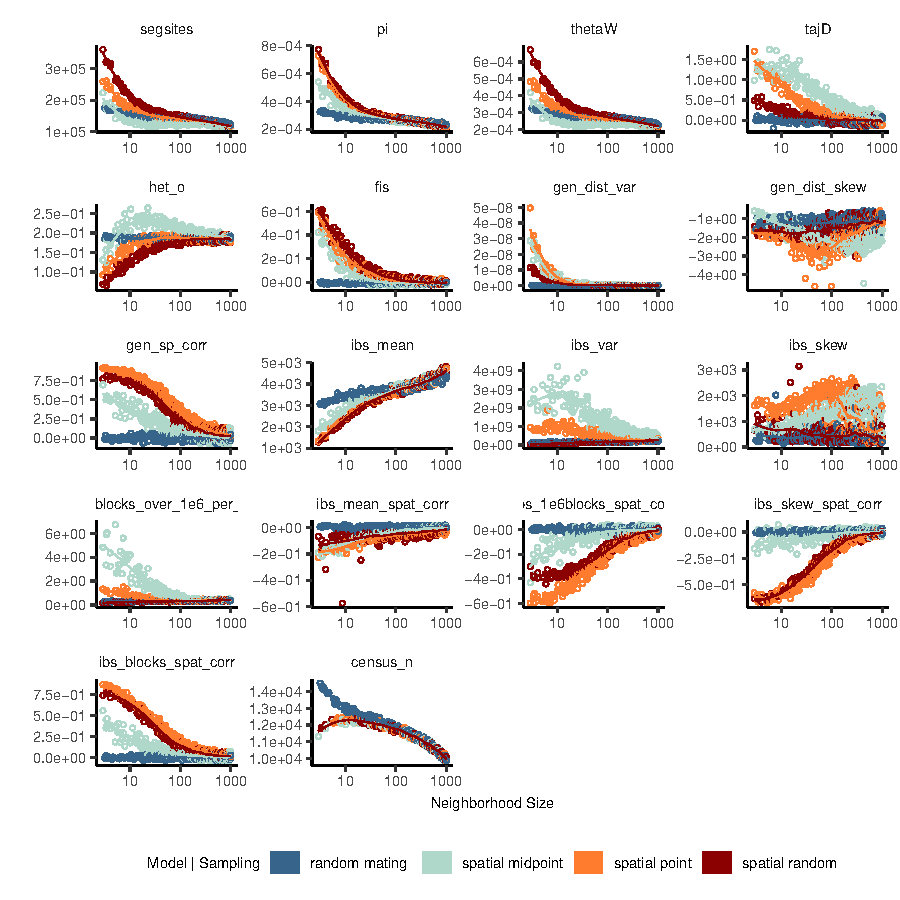
\includegraphics[width=\textwidth]{sumstats_by_neighbors.pdf}
\caption{[needs some polishing for labels etc] Summary statistics from spatial and random-mating SLiM simulations. Statistics are calculated from the genotype matrix of 60 randomly sampled individuals in each simulation.}
\label{fig:spectrum}
\end{figure*}

\afterpage{\clearpage}
\begin{figure*}[p]
\centering
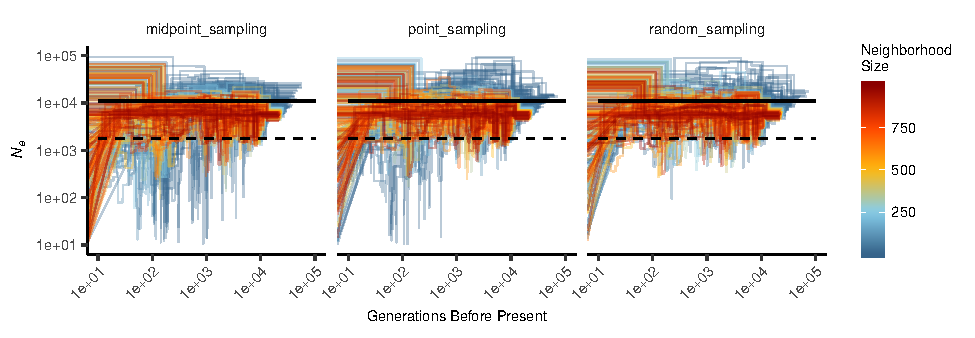
\includegraphics[width=\textwidth]{stairwayplot_by_sigma_facets.pdf}
\caption{Inferred demographic histories for spatial SLiM simulations from Stairwayplot. Lines shown are the median inferred $N_{e}$ across 100 bootstrap replicates for each simulation. Colors are scaled to Wright's neighborhood size (NS) and panels are divided by neighborhood size range. The black line is the census population size.}
\label{fig:spectrum}
\end{figure*}

\afterpage{\clearpage}
\begin{figure*}[p]
\centering
\includegraphics[width=\textwidth]{gwas_summary_nsig_qqplots_loglog.pdf}
\caption{Impacts of spatially correlated phenotypes and isolation by distance on linear regression GWAS. Colors represent different phenotype distributions as indicated in the figure legend. A: example phenotype distributions and sampling maps, with colors scaled to phenotype values. B: proportion of total variance explained by the first 10 PC axes, by neighborhood size. C: numbers of significant SNPs after FDR correction for linear-model GWAS conducted with (top) or without (bottom) PC covariates. D: Quantile-quantile plots of observed versus $p$ values relative to those expected from a uniform distribution. The dotted lines show the 95\% confidence region assuming binomial sampling and an alpha level of 0.05. Points above the 1:1 line reflect inflated -log10(p).}
\label{fig:spectrum}
\end{figure*}

\afterpage{\clearpage}

\bibliography{spaceness}

\end{document}









%%%%%%%%%%%%%%%%%%%%%%%%%%%%%%%%%%%%%%%%%%%%%%%%%%%%%%%%%%%%%%%%%%%%%%%%%%%%%


\section{Genetics Submission Guidelines}
Manuscripts submitted to \textit{GENETICS} should contain a clear description of the experimental design in sufficient detail so that the experimental analysis could be repeated by another scientist. If the level of detail necessary to explain the protocol goes beyond two paragraphs, give a short description in the main body of the paper and prepare a detailed description for supporting information.  For example, details would include indicating how many individuals were used, and if applicable how individuals or groups were combined for analysis. If working with mutants indicate how many independent mutants were isolated. If working with populations indicate how samples were collected and whether they were random with respect to the target population.


\subsection{Statistical Analysis} 

It is important to indicate what statistical analysis has been performed; not just the name of the software and options selected, but the method and model applied. In the case of many genes being examined simultaneously, or many phenotypes, a multiple comparison correction should be used to control the type I error rate, or a rationale for not applying a correction must be provided. The type of correction applied should be clearly stated. It should also be clear whether the p-values reported are raw, or after correction. Corrected p-values are often appropriate, but raw p-values should be available in the supporting materials so that others may perform their own corrections. In large scale data exploration studies (e.g. genome wide expression studies) a clear and complete description of the replication structure must be provided. 

\subsection{Data Availability}

At the end of the Materials and Methods section, include a statement on reagent and data availability. Please read the Data and Reagent Policy before writing the statement. Make sure to list the accession numbers or DOIs of any data you have placed in public repositories. List the file names and descriptions of any data you will upload as supplemental information. The statement should also include any applicable IRB numbers. You may include specifications for how to properly acknowledge or cite the data.

For example: Strains are available upon request. File S1 contains detailed descriptions of all supplemental files. File S2 contains SNP ID numbers and locations. File S3 contains genotypes for each individual. Sequence data are available at GenBank and the accession numbers are listed in File S3. Gene expression data are available at GEO with the accession number: GDS1234. Code used to generate the simulated data is provided in file S4. 


\section{Results and Discussion}

The results and discussion should not be repetitive. The results section should give a factual presentation of the data and all tables and figures should be referenced; the discussion should not summarize the results but provide an interpretation of the results, and should clearly delineate between the findings of the particular study and the possible impact of those findings in a larger context. Authors are encouraged to cite recent work relevant to their interpretations. Present and discuss results only once, not in both the Results and Discussion sections. It is sometimes acceptable to combine results and discussion. The text should be as succinct as possible. Heed Strunk and White's dictum: "Omit needless words!"

\section{Additional guidelines}

\subsection{Numbers} In the text, write out numbers nine or less except as part of a date, a fraction or decimal, a percentage, or a unit of measurement. Use Arabic numbers for those larger than nine, except as the first word of a sentence; however, try to avoid starting a sentence with such a number.

\subsection{Units} Use abbreviations of the customary units of measurement only when they are preceded by a number: "3 min" but "several minutes". Write "percent" as one word, except when used with a number: "several percent" but "75\%." To indicate temperature in centigrade, use ° (for example, 37°); include a letter after the degree symbol only when some other scale is intended (for example, 45°K).

\subsection{Nomenclature and Italicization} Italicize names of organisms even when  when the species is not indicated.  Italicize the first three letters of the names of restriction enzyme cleavage sites, as in HindIII. Write the names of strains in roman except when incorporating specific genotypic designations. Italicize genotype names and symbols, including all components of alleles, but not when the name of a gene is the same as the name of an enzyme. Do not use "+" to indicate wild type. Carefully distinguish between genotype (italicized) and phenotype (not italicized) in both the writing and the symbolism.

\subsection{Cross References}
Use the \verb|\nameref| command with the \verb|\label| command to insert cross-references to section headings. For example, a \verb|\label| has been defined in the section \nameref{sec:materials:methods}.

\section{In-text Citations}

Add citations using the \verb|\citep{}| command, for example \citep{neher2013genealogies} or for multiple citations, \citep{neher2013genealogies, rodelsperger2014characterization,Falush16}

\section{Examples of Article Components}
\label{sec:examples}

The sections below show examples of different header levels, which you can use in the primary sections of the manuscript (Results, Discussion, etc.) to organize your content.

\section{First level section header}

Use this level to group two or more closely related headings in a long article.

\subsection{Second level section header}

Second level section text.

\subsubsection{Third level section header:}

Third level section text. These headings may be numbered, but only when the numbers must be cited in the text. 

\section{Figures and Tables}

Figures and Tables should be labelled and referenced in the standard way using the \verb|\label{}| and \verb|\ref{}| commands.

\subsection{Sample Figure}

Figure \ref{fig:spectrum} shows an example figure.

\begin{figure}[htbp!]
\centering
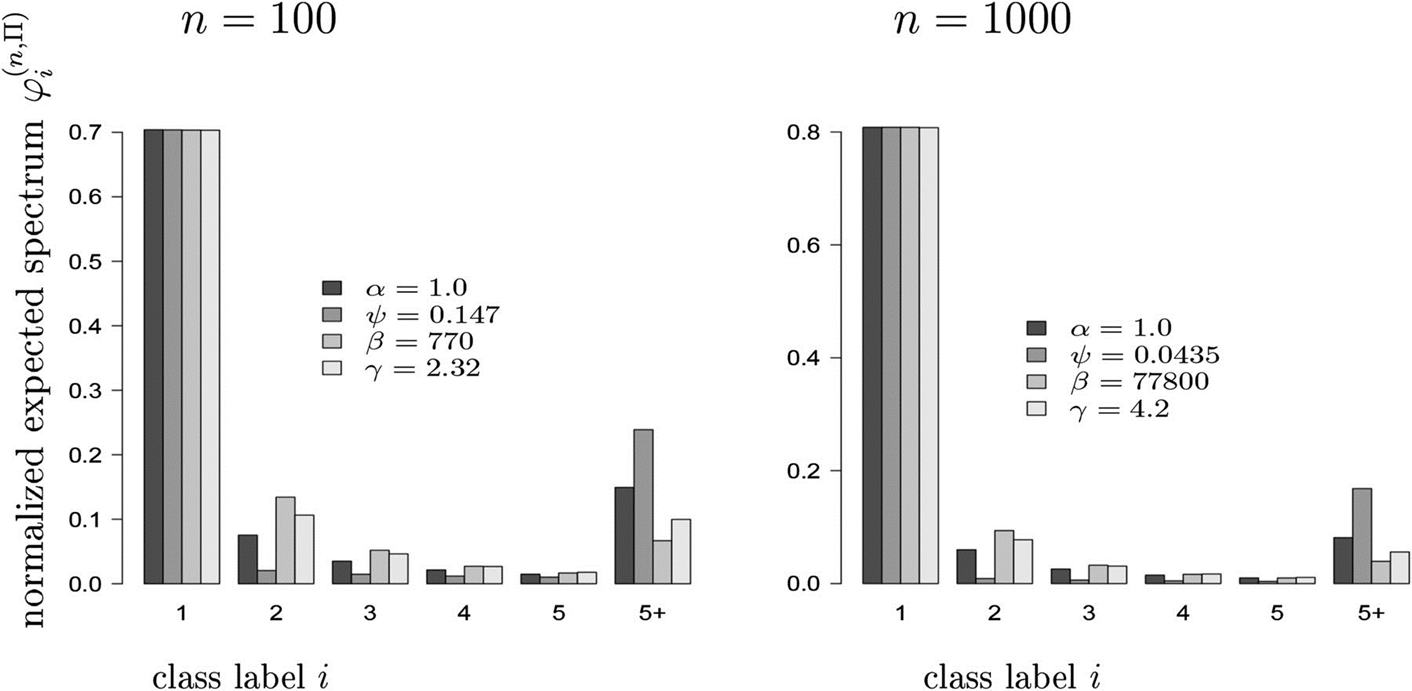
\includegraphics[width=\linewidth]{example-figure}
\caption{Example figure from \url{10.1534/genetics.114.173807}. Please include your figures in the manuscript for the review process. You can upload figures to Overleaf via the Project menu. Upon acceptance, we'll ask for your figure files to be uploaded in any of the following formats: TIFF (.tiff), JPEG (.jpg), Microsoft PowerPoint (.ppt), EPS (.eps), or Adobe Illustrator (.ai).  Images should be a minimum of 300 dpi in resolution and 500 dpi minimum if line art images.  RGB, CMYK, and Grayscale are all acceptable. Halftones should be high contrast with sharp detail, because some loss of detail and contrast is inevitable in the production process. Figures should be 10-20 cm in width and 1-25 cm in height. Graph axes must be exactly perpendicular and all lines of equal density.
Label multiple figure parts with A, B, etc. in bolded type, and use Arrows and numbers to draw attention to areas you want to highlight. Legends should start with a brief title and should be a self-contained description of the content of the figure that provides enough detail to fully understand the data presented. All conventional symbols used to indicate figure data points are available for typesetting; unconventional symbols should not be used. Italicize all mathematical variables (both in the figure legend and figure) , genotypes, and additional symbols that are normally italicized.  
}%
\label{fig:spectrum}
\end{figure}

\subsection{Sample Video}

Figure \ref{video:spectrum} shows how to include a video in your manuscript.

\begin{figure}[htbp]
\centering
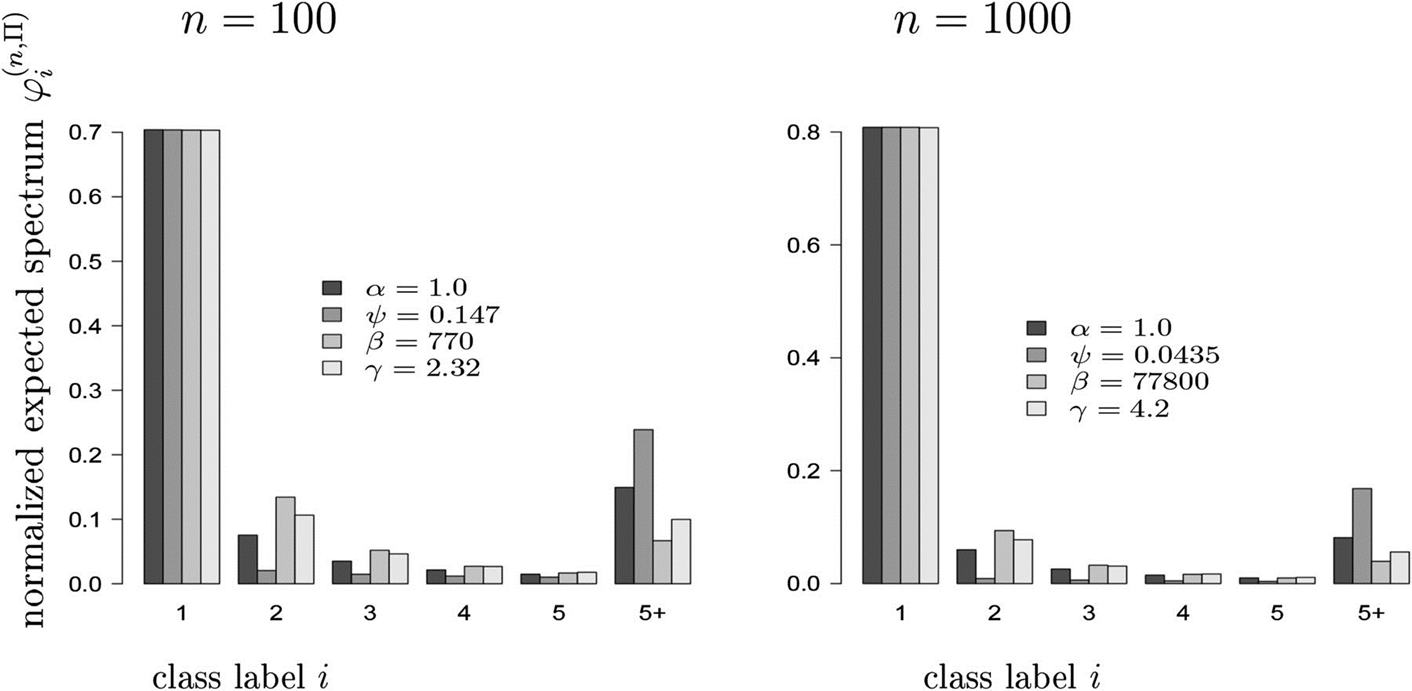
\includegraphics[width=\linewidth]{example-figure}
\caption{Example movie (the figure file above is used as a placeholder for this example). \textit{GENETICS} supports video and movie files that can be linked from any portion of the article - including the abstract. Acceptable formats include .asf, avi, .wav, and all types of Windows Media files.   
}%
\label{video:spectrum}
\end{figure}


\subsection{Sample Table}

Table \ref{tab:shape-functions} shows an example table. Avoid shading, color type, line drawings, graphics, or other illustrations within tables. Use tables for data only; present drawings, graphics, and illustrations as separate figures. Histograms should not be used to present data that can be captured easily in text or small tables, as they take up much more space.  

Tables numbers are given in Arabic numerals. Tables should not be numbered 1A, 1B, etc., but if necessary, interior parts of the table can be labeled A, B, etc. for easy reference in the text.  


\begin{table*}[htbp]
\centering
\caption{\bf Students and their grades}
\begin{tableminipage}{\textwidth}
\begin{tabularx}{\textwidth}{XXXX}
\hline
Student & Grade\footnote{This is an example of a footnote in a table. Lowercase, superscript italic letters (a, b, c, etc.) are used by default. You can also use *, **, and *** to indicate conventional levels of statistical significance, explained below the table.} & Rank & Notes \\
\hline
Alice & 82\% & 1 & Performed very well.\\
Bob & 65\% & 3 & Not up to his usual standard.\\
Charlie & 73\% & 2 & A good attempt.\\
\hline
\end{tabularx}
  \label{tab:shape-functions}
\end{tableminipage}
\end{table*}

\section{Sample Equation}

Let $X_1, X_2, \ldots, X_n$ be a sequence of independent and identically distributed random variables with $\text{E}[X_i] = \mu$ and $\text{Var}[X_i] = \sigma^2 < \infty$, and let
\begin{equation}
S_n = \frac{X_1 + X_2 + \cdots + X_n}{n}
      = \frac{1}{n}\sum_{i}^{n} X_i
\label{eq:refname1}
\end{equation}
denote their mean. Then as $n$ approaches infinity, the random variables $\sqrt{n}(S_n - \mu)$ converge in distribution to a normal $\mathcal{N}(0, \sigma^2)$.